\documentclass{article}
\usepackage{polski}
\usepackage[T1]{fontenc}
\usepackage[utf8x]{inputenc}
\usepackage{booktabs}
\usepackage{multirow}
\usepackage{graphicx}
\usepackage{textcomp}
\usepackage{eurosym}
\usepackage{float}
\usepackage{adjustbox}
\usepackage{graphics}
\usepackage{tabularx}
\usepackage{rotating}
\usepackage{tabulary}
\usepackage{listings}
\usepackage{amstext}
\usepackage{xcolor}
\usepackage{url,textcomp}
\usepackage{hyperref}
\usepackage[framed,numbered,autolinebreaks,useliterate]{mcode}
\usepackage{listings}
\usepackage{xcolor}
\lstset { 
language=C++,
backgroundcolor=\color{black!5}, % set backgroundcolor
basicstyle=\footnotesize,% basic font setting
}



\title{Projektowanie algorytmów i metody sztucznej inteligencji - Raport 1}

\author{Damian Ryś}

 
\begin{document}

\maketitle


\tableofcontents
\section{Wstęp}
Grupa lab: E12-93c zmien

Termin zajęć: PN 18:45-20:35

Numer indeksu: 252936

Prowadzący: Dr inż. Piotr Ciskowski
\newpage
\section{Zadanie}
Postawionym pzed nami problemem jest wysłanie przez użytkownika A do użytkownika B wiadomości przez Internet.
wiadomość ta powinna zostać wysłana w serii pakietów na komputer użytkownika B.
Problem polega w tym, że pakiety mogą przychodzić z różnych przycznym w losowej kolejności do użytkownika B.
Nasz program powinien zatem:
\begin{enumerate}
    \item Podzielić naszą wiadomość na szereg pakietów
    \item Przelosować pakiety w celu zasymulowania sytuacji
    \item Wczytać do struktury danych nasze pakiety
    \item Przesyłać pakiety w foramcie [klucz,wartość]
    \begin{enumerate}
        \item klucz powininen mieć unikalną wartość
        \item wartość powinna być dowolnego typu (użytkownik powinine mieć możliwość przesłania dowolnej wiadomości)
    \end{enumerate}
    \item Złączyć wiadomość w jedną,prawidłową całość i wyświetlić użytkownikowi
\end{enumerate}
\section{Kolejka Priorytetowa}
Wobec postawionego problemu strukturą ADT, którą wybrałem jest kolejka priorytetowa bazowana na liście.
\subsection{Czym jest kolejka priorytetowa?}
Kolejka priorytetowa (ang. priority queue) jest kolejką, w której elementy są ułożone nie w kolejności wprowadzania, lecz w kolejności priorytetu.
Każdy element kolejki posiada dodatkowe pole priority, w którym przechowuje swój priorytet – czyli ważność.
Gwarantuje to pobieranie z kolejki jako pierwszych elementów o najwyższym priorytecie. 
Elementy o priorytetach niższych zostaną pobrane dopiero wtedy, gdy zostaną usunięte wszystkie elementy o priorytetach wyższych.


\subsection{Zalety i wady}
Strukturę tą wybrałem ze względu na:
\begin{itemize}
    \item Łatwość implementacji
    \item Złożoność czasową lepszą niż O(n) dla uzyskania min oraz max
    \item Dynamiczną alokację danych
\end{itemize}


\subsection{Implementacja}

\begin{lstlisting}
    template<typename T>
    class PriorityQueue
    {
        typedef struct Node
        {
            T field; //wartosc 
            int key; // klucz
            Node *nextNode; 
        } *nodePointer;
    
        nodePointer front; //wskaznik na nastepny element
        nodePointer back; // wskaznik na poprzedni element
    public:
        PriorityQueue(); //konstruktor
        ~PriorityQueue(); //destruktor
        // dodanie elementu
        void enqueue(const T& newElement, int priority); 
        // usuniecie elementu
        void dequeue(); 
        // wyswietlenie kolejki w prawidlowym porzadku
        void Print(); 
        // sprawdzenie czy kolejka nie jest pusta
        bool Empty(); 
    private:
    //metody do obslugi enqueue i dequeue
        void pushBack(const T& newElement, int priority); 
        void pushFront(const T& newElement, int priority);
        void pushFirstNode(const T& newElement, int priority);
        void pushInside(const T& newElement, int priority);
        
    };
    \end{lstlisting}
    
Powyżej znajduję się klasa kolejki priorytowej, reszta kodu dostępna jest na 
rezpozytorium na \href{https://github.com/Damiry0/PAMSI}{Githubie} lub dołączonym skompresowanym pliku.
\newpage
\subsection{Złożoności obliczeniowe}
Dla naszego programu zgodnie z załozeniami projektowymi zostały obliczene złożoności czasowe poszczególnych 
funkcji naszej struktury:


\begin{figure}[H]
    \centering
    \hspace*{-1cm}
    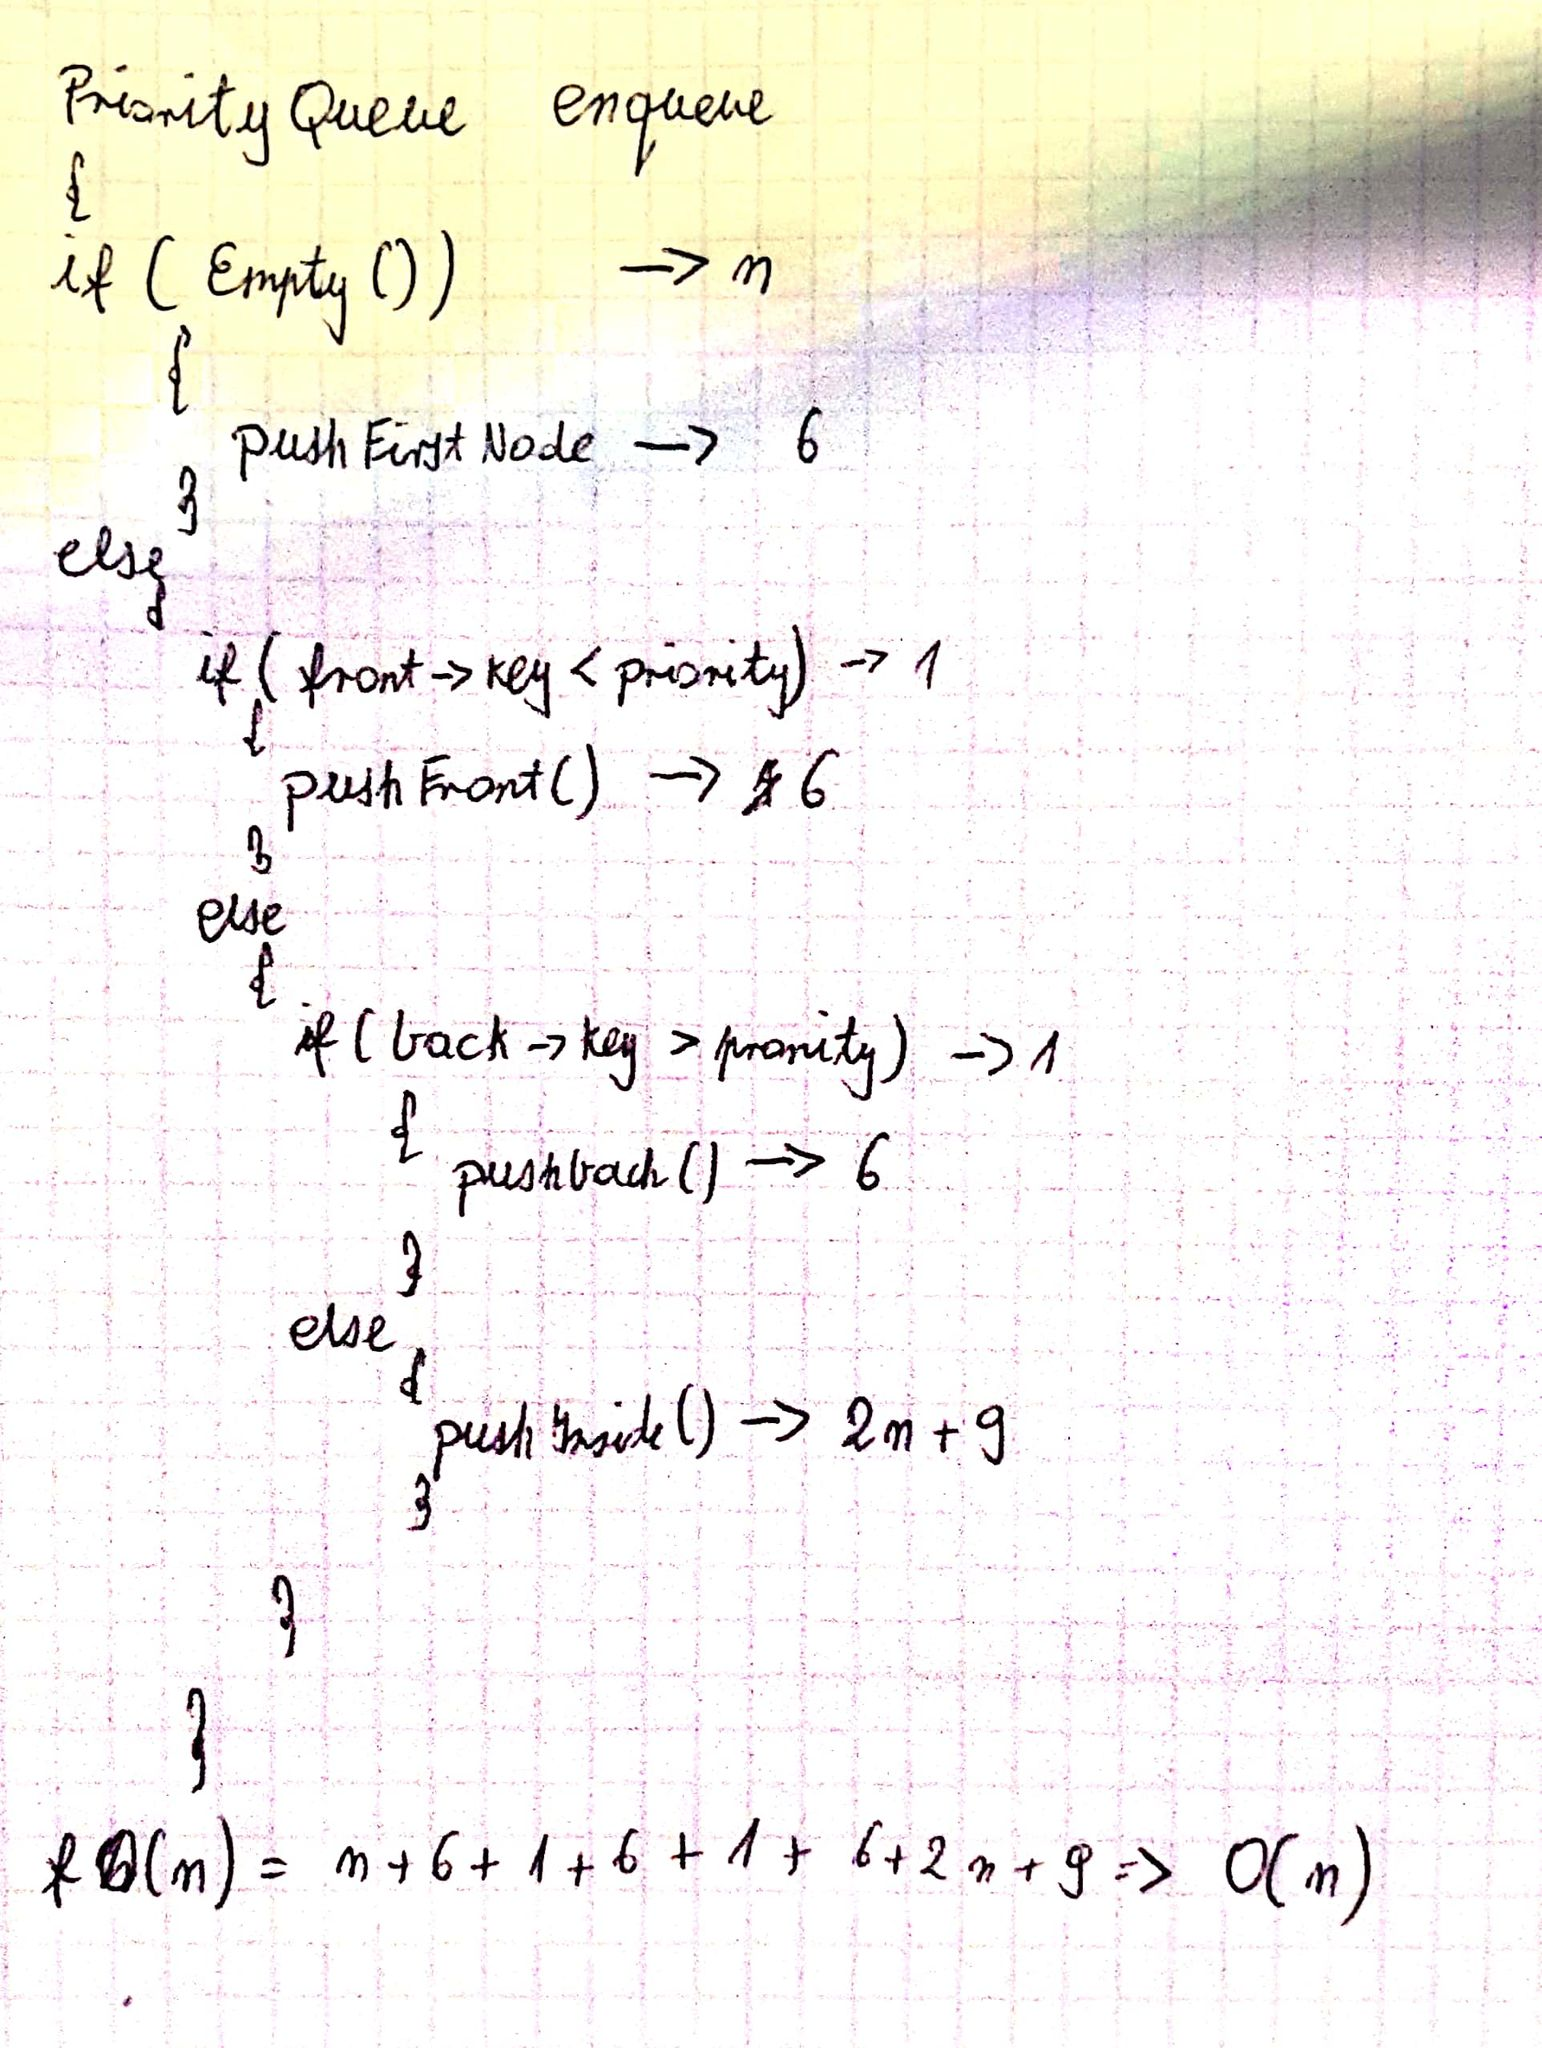
\includegraphics[totalheight=10cm]{zlozonosc.jpg}
    \caption{Złożoność obliczeniowa dla metody enqueue}
    \label{2}
\end{figure}

Złożoność została policzona również dla innych metod,co można zobaczyć w tabelce poniżej:

//tabelka

Nasze wyniki pokrywają się z danymi dostępnymi w internecie,jak na przykład 
\href{https://eduinf.waw.pl/inf/alg/001_search/0106.php}{TUTAJ}. Uznaje zatem,
że kolejka została zaimplementowana poprawnie.


\subsection{Testy}
Dla bazy naszych testów zasymulowałem sytuacje w której użytkownik B otrzymuje od
użytkownika A pakiety w złej kolejności.

\begin{figure}[H]
    \centering
    \hspace*{-1cm}
    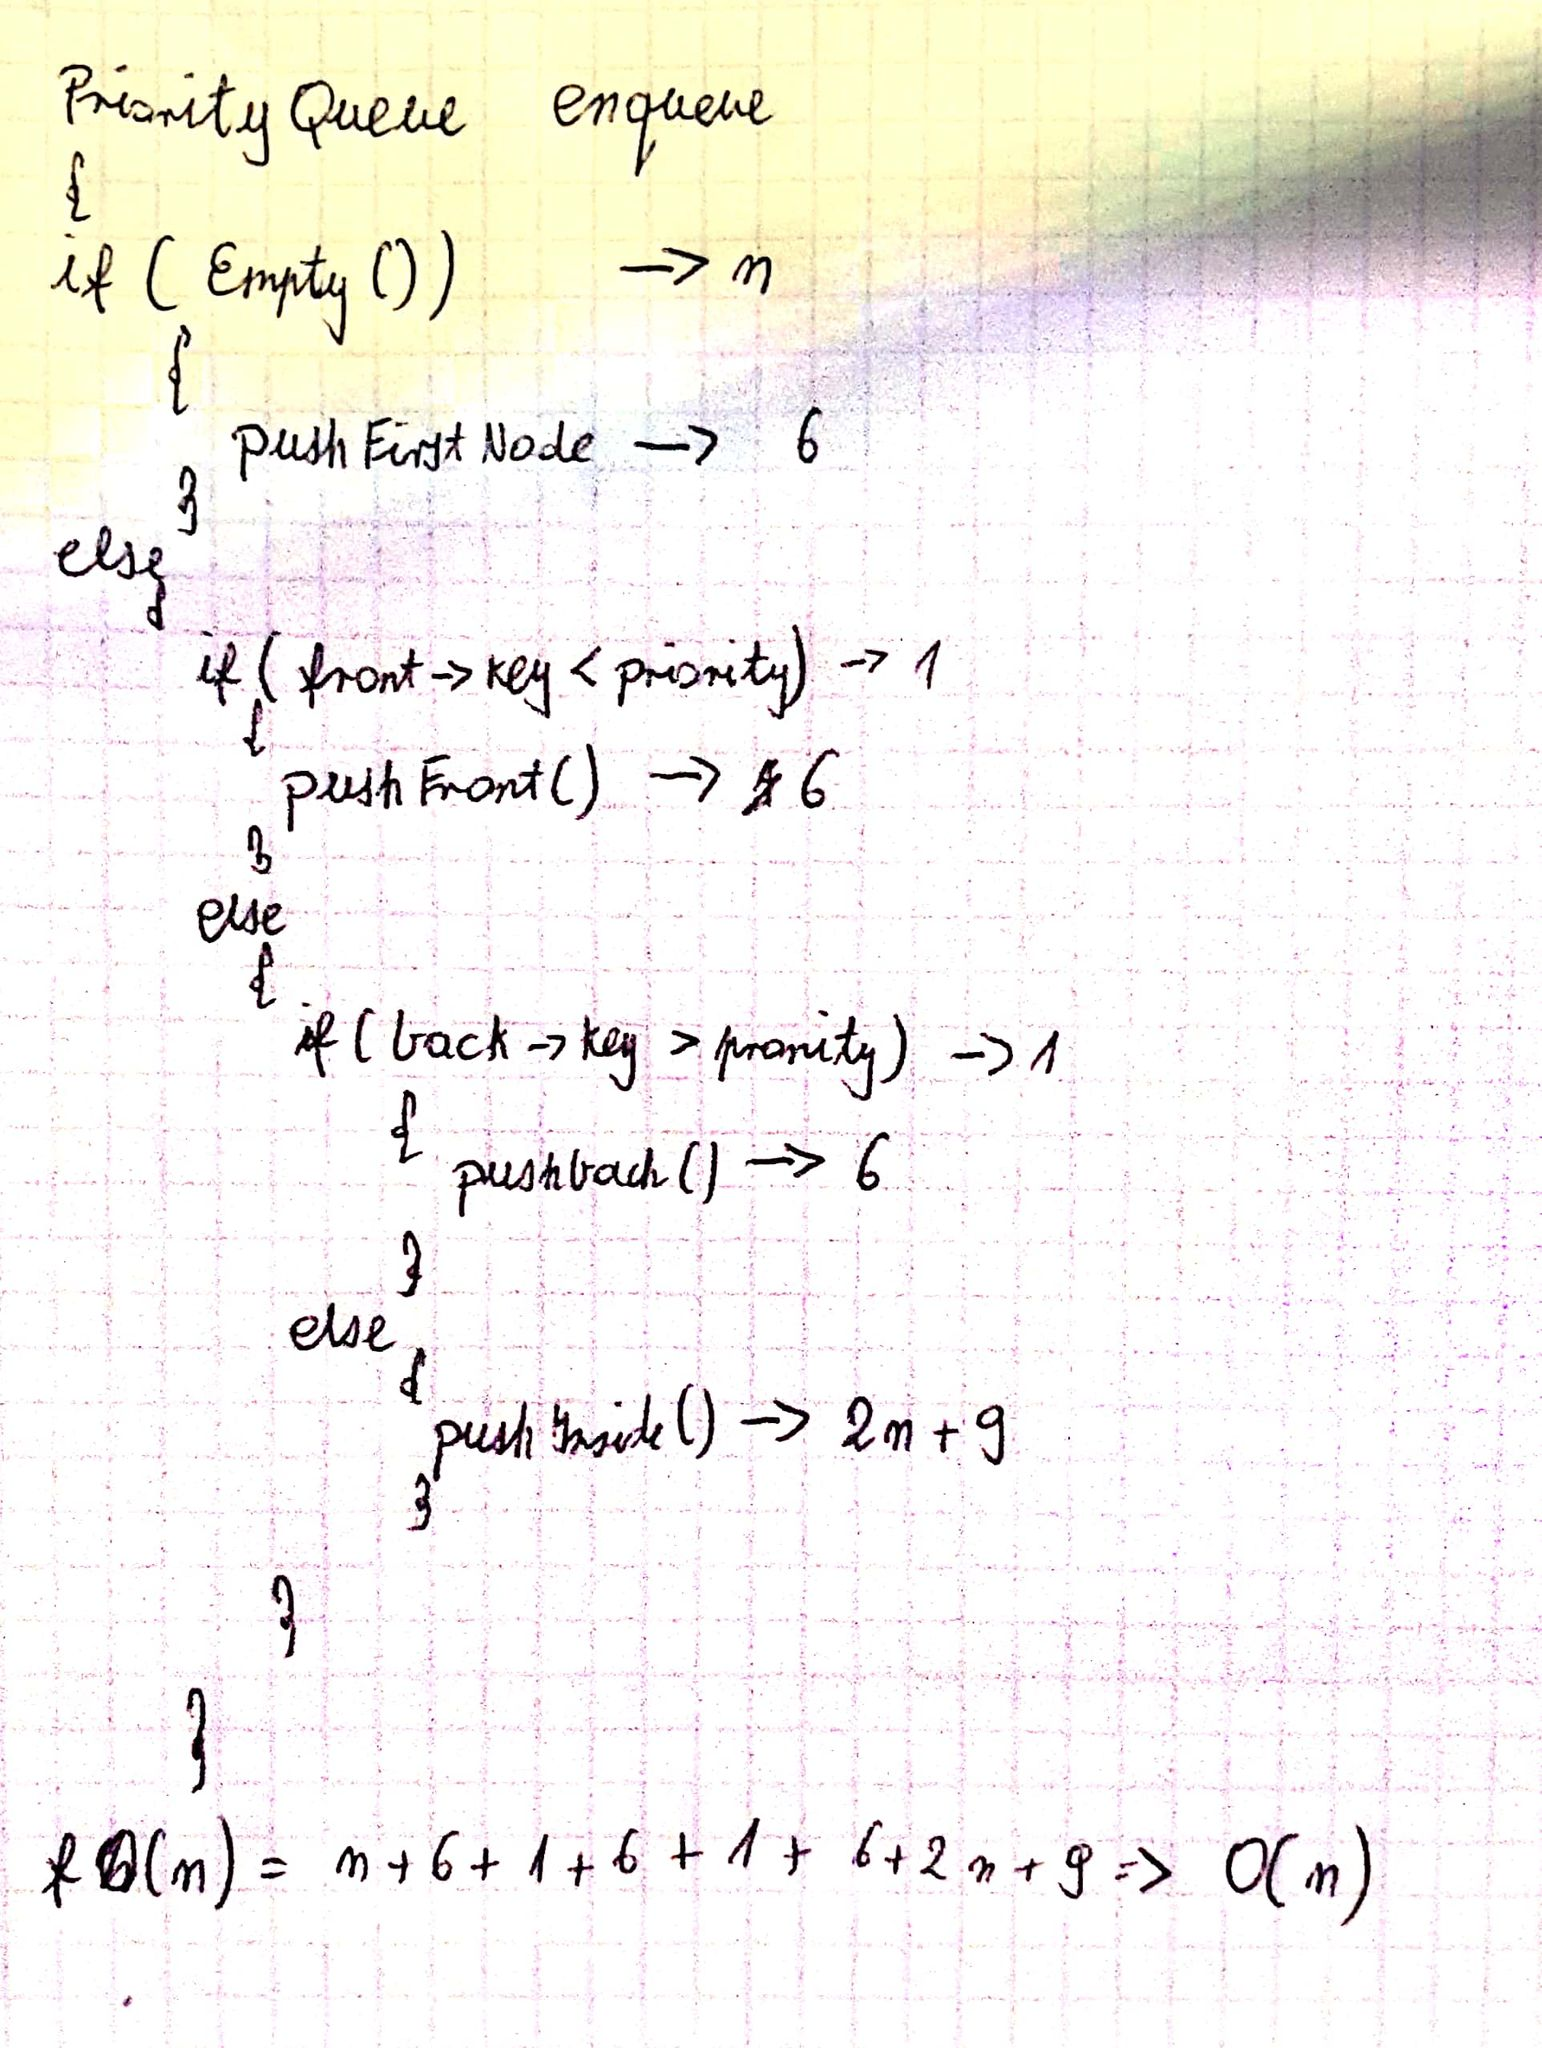
\includegraphics[totalheight=8cm]{zlozonosc.jpg}
    \caption{Złożoność obliczeniowa dla metody enqueue}
    \label{2}
\end{figure}

Program został przetestowany również dla różnego typu elementów, co widać na 
poniższym screenie:

\begin{figure}[H]
    \centering
    \hspace*{-1cm}
    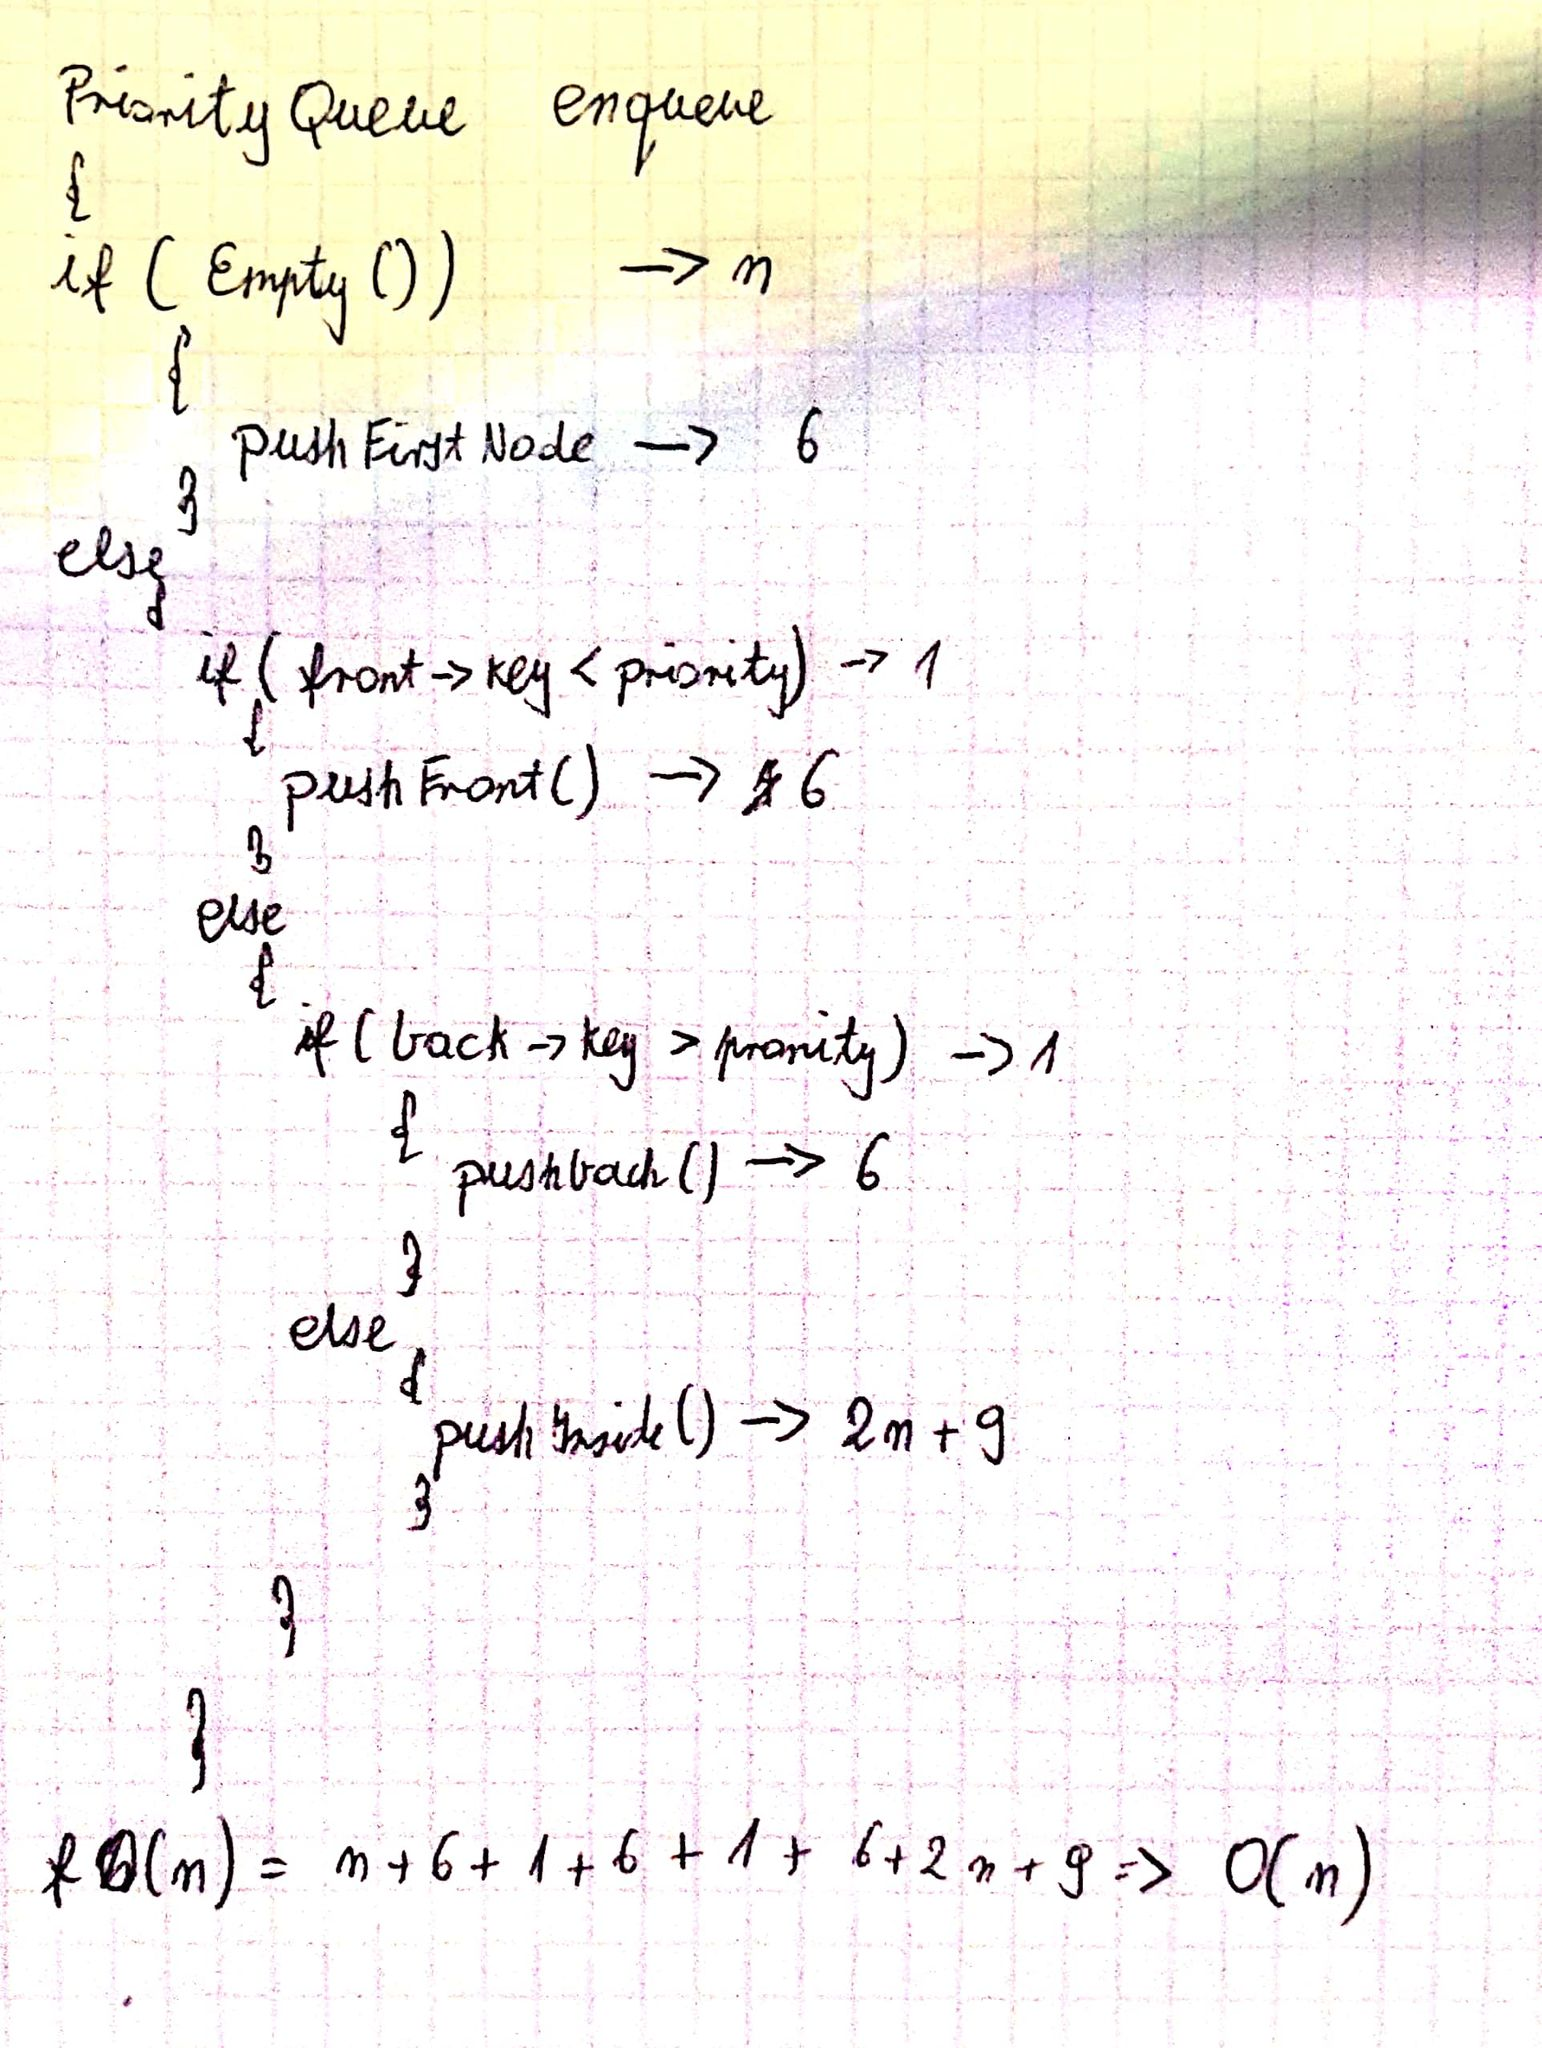
\includegraphics[totalheight=8cm]{zlozonosc.jpg}
    \caption{Złożoność obliczeniowa dla metody enqueue}
    \label{2}
\end{figure}


Program finalnie przeszedł testy, zatem uznaje, że program działa prawidłowo.

\section{Wnioski}
\section{Bibliografia}
\href{https://eduinf.waw.pl/inf/alg/001_search/0106.php}{Schemat implementacji wraz z schematami blokowymi}

\href{https://bradfieldcs.com/algos/trees/priority-queues-with-binary-heaps/}{Inne rozwiązanie problemu na drzewach binarnych}

\href{https://www.hackerearth.com/practice/notes/heaps-and-priority-queues/}{Złożoności czasowe różnych algorytmów}
\end{document}